\documentclass[11pt]{article}
\usepackage[margin=1in]{geometry}
\usepackage{enumitem}
\usepackage{tabularx}
\usepackage{booktabs}
\usepackage{tikz}
\setlist{nosep}
\setlength{\parindent}{0pt}
\setlength{\parskip}{4pt}

\definecolor{accent}{RGB}{37,99,235}
\definecolor{good}{RGB}{22,163,74}
\definecolor{next}{RGB}{234,88,12}
\definecolor{phone}{RGB}{24,24,27}
\definecolor{video}{RGB}{63,63,70}

\title{AR Sudoku: App and Website Design}
\author{Muhammad Ali Hassan}
\date{}

\begin{document}
\maketitle

\section{Goal}

Point any phone or laptop camera at a printed Sudoku. The website finds the puzzle, solves it, and
writes the missing digits on the paper. It also works on a puzzle you already started: it checks
your handwritten digits and fills in the rest.
\begin{itemize}
  \item \textbf{Leonardo:} vision and solver (\texttt{sudoku\_cv}).
  \item \textbf{Me:} the website. Camera, screens, drawing the digits on the paper, free hosting.
\end{itemize}
Classical computer vision only, no neural networks.

\section{Screens}

\begin{figure}[h]
\centering
% ---------- Home screen ----------
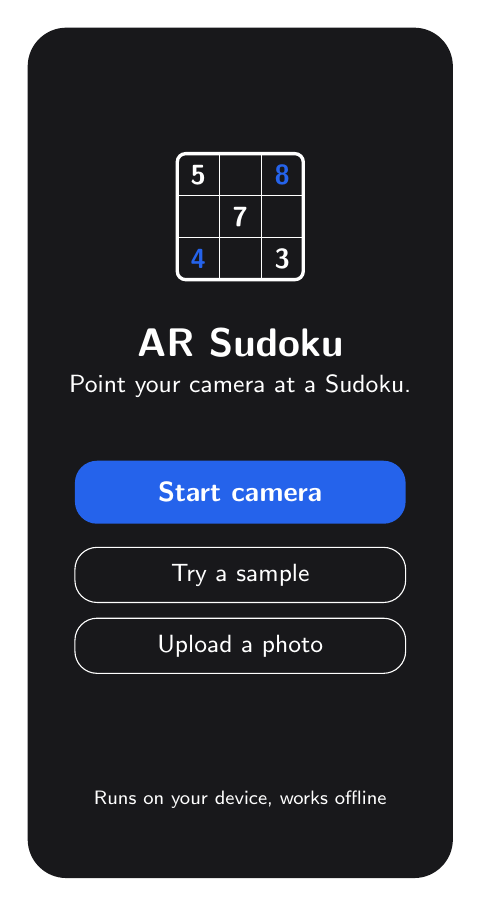
\begin{tikzpicture}[font=\sffamily]
  \fill[phone, rounded corners=14pt] (0,0) rectangle (5.4,10.8);
  % grid icon
  \begin{scope}[shift={(1.9,7.6)}]
    \draw[white, line width=1.2pt, rounded corners=3pt] (0,0) rectangle (1.6,1.6);
    \foreach \i in {1,2} {
      \draw[white!60] (\i*0.5333,0) -- (\i*0.5333,1.6);
      \draw[white!60] (0,\i*0.5333) -- (1.6,\i*0.5333);
    }
    \node[white, font=\sffamily\bfseries] at (0.2667,1.3333) {5};
    \node[accent, font=\sffamily\bfseries] at (1.3333,1.3333) {8};
    \node[white, font=\sffamily\bfseries] at (0.8,0.8) {7};
    \node[accent, font=\sffamily\bfseries] at (0.2667,0.2667) {4};
    \node[white, font=\sffamily\bfseries] at (1.3333,0.2667) {3};
  \end{scope}
  \node[white, font=\sffamily\bfseries\Large] at (2.7,6.8) {AR Sudoku};
  \node[white!65, font=\sffamily\small] at (2.7,6.25) {Point your camera at a Sudoku.};
  % buttons
  \fill[accent, rounded corners=8pt] (0.6,4.5) rectangle (4.8,5.3);
  \node[white, font=\sffamily\bfseries] at (2.7,4.9) {Start camera};
  \draw[white!60, rounded corners=8pt] (0.6,3.5) rectangle (4.8,4.2);
  \node[white, font=\sffamily\small] at (2.7,3.85) {Try a sample};
  \draw[white!60, rounded corners=8pt] (0.6,2.6) rectangle (4.8,3.3);
  \node[white, font=\sffamily\small] at (2.7,2.95) {Upload a photo};
  \node[white!55, font=\sffamily\scriptsize] at (2.7,1.0) {Runs on your device, works offline};
\end{tikzpicture}
\hspace{1.2cm}
% ---------- Camera screen ----------
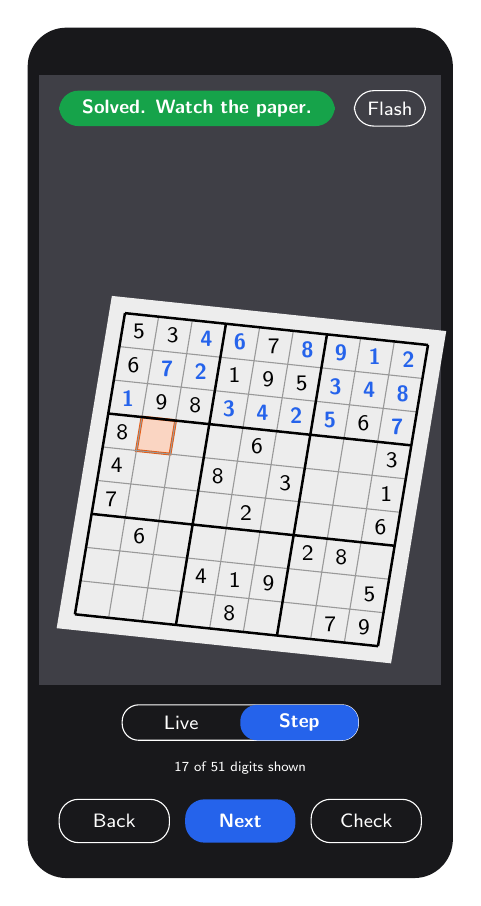
\begin{tikzpicture}[font=\sffamily]
  \fill[phone, rounded corners=14pt] (0,0) rectangle (5.4,10.8);
  \fill[video] (0.15,2.45) rectangle (5.25,10.2);
  % status pill
  \fill[good, rounded corners=7pt] (0.4,9.55) rectangle (3.9,10.0);
  \node[white, font=\sffamily\bfseries\scriptsize] at (2.15,9.775) {Solved. Watch the paper.};
  \draw[white!60, rounded corners=7pt] (4.15,9.55) rectangle (5.05,10.0);
  \node[white, font=\sffamily\scriptsize] at (4.6,9.775) {Flash};
  % the paper with the puzzle, slightly turned
  \begin{scope}[shift={(0.6,3.35)}, rotate=-6, xslant=0.06]
    \fill[white!93!black] (-0.2,-0.2) rectangle (4.07,4.07);
    \def\s{0.43}
    % next cell to reveal (row 3, column 1)
    \fill[next!25] (1*\s,5*\s) rectangle (2*\s,6*\s);
    \draw[next, line width=1pt] (1*\s,5*\s) rectangle (2*\s,6*\s);
    \foreach \i in {1,2,4,5,7,8} {
      \draw[black!40] (\i*\s,0) -- (\i*\s,9*\s);
      \draw[black!40] (0,\i*\s) -- (9*\s,\i*\s);
    }
    \foreach \i in {0,3,6,9} {
      \draw[black, line width=0.9pt] (\i*\s,0) -- (\i*\s,9*\s);
      \draw[black, line width=0.9pt] (0,\i*\s) -- (9*\s,\i*\s);
    }
    % printed digits
    \foreach \row [count=\r from 0] in {
      {5,3,0,0,7,0,0,0,0},{6,0,0,1,9,5,0,0,0},{0,9,8,0,0,0,0,6,0},
      {8,0,0,0,6,0,0,0,3},{4,0,0,8,0,3,0,0,1},{7,0,0,0,2,0,0,0,6},
      {0,6,0,0,0,0,2,8,0},{0,0,0,4,1,9,0,0,5},{0,0,0,0,8,0,0,7,9}} {
      \foreach \d [count=\c from 0] in \row {
        \ifnum\d>0
          \node[black, font=\sffamily\footnotesize] at (\c*\s+0.5*\s, 8.5*\s-\r*\s) {\d};
        \fi
      }
    }
    % digits already revealed by the app
    \foreach \row [count=\r from 0] in {
      {0,0,4,6,0,8,9,1,2},{0,7,2,0,0,0,3,4,8},{1,0,0,3,4,2,5,0,7}} {
      \foreach \d [count=\c from 0] in \row {
        \ifnum\d>0
          \node[accent, font=\sffamily\bfseries\footnotesize] at (\c*\s+0.5*\s, 8.5*\s-\r*\s) {\d};
        \fi
      }
    }
  \end{scope}
  % controls
  \draw[white!50, rounded corners=6pt] (1.2,1.75) rectangle (4.2,2.2);
  \fill[accent, rounded corners=6pt] (2.7,1.75) rectangle (4.2,2.2);
  \node[white!80, font=\sffamily\scriptsize] at (1.95,1.975) {Live};
  \node[white, font=\sffamily\bfseries\scriptsize] at (3.45,1.975) {Step};
  \node[white!65, font=\sffamily\tiny] at (2.7,1.4) {17 of 51 digits shown};
  \draw[white!60, rounded corners=7pt] (0.4,0.45) rectangle (1.8,1.0);
  \node[white, font=\sffamily\scriptsize] at (1.1,0.725) {Back};
  \fill[accent, rounded corners=7pt] (2.0,0.45) rectangle (3.4,1.0);
  \node[white, font=\sffamily\bfseries\scriptsize] at (2.7,0.725) {Next};
  \draw[white!60, rounded corners=7pt] (3.6,0.45) rectangle (5.0,1.0);
  \node[white, font=\sffamily\scriptsize] at (4.3,0.725) {Check};
\end{tikzpicture}

\vspace{4pt}
\small Home screen \hspace{3.6cm} Camera screen in Step mode
\end{figure}

\begin{itemize}
  \item \textbf{Home:} start the camera, try a sample puzzle, or upload a photo.
  \item \textbf{Camera:} a message on top tells the user what to do. Digits appear on the paper and
        stay on it when the paper moves. Printed digits are black, the app's digits are blue, the
        next one is orange.
  \item \textbf{Live or Step:} Live shows all missing digits one after another. Step shows one per
        tap, so it works as a hint.
  \item \textbf{Check:} if a digit was read wrong, the user freezes the picture and taps to fix it.
  \item \textbf{Continue mode:} the user's handwritten digits get green when right, red when wrong.
\end{itemize}

\begin{tabularx}{\textwidth}{@{}lX@{}}
\toprule
What the code reports & Message on screen \\
\midrule
no puzzle found & Point the camera at a Sudoku \\
puzzle found, reading & Hold still\dots \\
can't be solved & Some digits look wrong. Tap Check. \\
solved & Solved. Watch the paper. \\
\bottomrule
\end{tabularx}

\section{How it works}

\begin{enumerate}
  \item The camera gives a stream of video frames.
  \item Whenever it is free, the site takes the newest frame, shrinks it to 640\,px, and gives it to
        Leonardo's code. His Python runs inside the browser with Pyodide, in a background thread, so
        the video never freezes.
  \item His code returns the puzzle's 4 corners, the digits, the solution and the order to show them.
  \item The site writes the digits on a flat square and bends it onto the paper with the homography
        (a CSS \texttt{matrix3d} transform).
\end{enumerate}
There is no server: nothing to pay for, the video never leaves the phone, and the site works offline
after the first visit. It is hosted for free on GitHub Pages. My code lives in \texttt{app/}.

If this is too slow on phones: use smaller frames (480\,px), or track the corners with OpenCV.js, or
as a last resort run the Python on a free Hugging Face server.

\section{What I need from Leonardo}

\begin{itemize}
  \item A \texttt{solve(givens)} function, to solve again after the user fixes a digit.
  \item For Continue mode: handwritten digits kept apart from printed ones, plus a list of wrong
        ones. Handwriting can be read classically with HOG features and k-nearest neighbours on
        MNIST digits.
  \item A confidence score per cell, so the Check screen can shade doubtful cells.
  \item Optional: the in-between images (threshold, contour, flat grid) for a ``How it works'' demo.
\end{itemize}

\section{Steps to finish}

\begin{tabularx}{\textwidth}{@{}l>{\raggedright\arraybackslash}p{2.1cm}X@{}}
\toprule
& Dates & What I do \\
\midrule
1 & by Nov 2 & Run Pyodide + OpenCV on a laptop, an iPhone and an Android phone and time it. Put a
  test page on GitHub Pages. Decide if the in-browser plan is fast enough. \\
2 & Nov 3 -- 9 & Camera on all devices. Send frames to the background thread. Draw the digits from
  Leonardo's stub onto the sample photos. \\
3 & Nov 10 -- 15 & All screens: home, messages, Live and Step, Check, Continue colours, photo
  upload, offline install. \\
4 & Nov 16 -- 22 & Swap the stub for Leonardo's real code. Test on the sample photos. \\
5 & Nov 23 -- 30 & Test on the 3 devices, let 5 classmates try it, fix problems. Code freeze Nov 30. \\
6 & Dec 1 -- 11 & Demo on Dec 1 or 3 with a backup video. Report due Dec 11. \\
\bottomrule
\end{tabularx}

\section{Testing}

On a laptop, an iPhone and an Android phone:
\begin{itemize}
  \item \textbf{Speed:} digit updates per second (target: 15 on a laptop, 10 on phones).
  \item \textbf{Load time:} under 10\,s the first time, under 2\,s after.
  \item \textbf{Time to solve:} from ``Start camera'' to solved, on 10 printed puzzles.
  \item \textbf{Steadiness:} how much the digits shake while the paper is still.
  \item \textbf{Continue mode:} on 10 half-filled puzzles, how many wrong digits are caught.
  \item \textbf{Ease of use:} 5 classmates try it with no help.
\end{itemize}

\section{Risks}

\begin{itemize}
  \item \textbf{Too slow on phones:} the fallbacks in section 3.
  \item \textbf{Handwriting read wrong:} the user fixes it on the Check screen.
  \item \textbf{iPhone camera issues:} test on a real iPhone in week 1; photo upload always works.
  \item \textbf{Demo fails in class:} recorded backup video.
\end{itemize}

\end{document}
